\setchapterpreamble[u]{\margintoc}

\chapter{Propiedades de los grupos de homología}
En este capítulo, introducimos algunas de las propiedades de los grupos de
homología. Estas propiedades son suficientes para calcular la homología de muchos
espacios, utilizando una secuencia exacta conocida como la \textbf{secuencia de
Mayer-Vietoris}, que presentaremos en el \refch{MVTema}.

\section{Axioma de la dimensión}
Sea $X=\{\star\}$. Dado un $n \geq 0$, existirá un único $n$-símplice singular
$\phi_n\colon\sigma_n \to X$, que envía a todos los puntos de
$\sigma_n$ en $\star$. Las caras de un $n$-símplice singular son $(n-1)$-símplice
singulares; sin embargo, acabamos de ver que el único $(n-1)$-símplice singular
es la aplicación constante, por lo que las caras de $\phi_n$ son $\phi_{n-1}$.
Por tanto,
\begin{align*}
\p\phi_n=\sum^n_{i=0}(-1)^i\p_{(i)}\phi_{n}=\sum^n_{i=0}(-1)^i\phi_{n-1}=
\begin{cases}
\phi_{n-1}	&\mbox{ si }n\mbox{ es par}\\
0          	&\mbox{ si }n\mbox{ es impar}
\end{cases}
\end{align*}

Dado que $S_n(X)=\la \phi_n\ra$, el operador borde $\p_n\colon S_n(X)
\to S_{n-1}(X)$ es un isomorfismo si $n$ es par y cero si $n$ es impar. Por tanto, para
$n > 0$,
\[\begin{array}{rcl}
Z_{2n+1}(X)\cong B_{2n+1}(X)&\implies& H_{2n+1}(X)=0\\[4pt]
Z_{2n}(X)=0=B_{2n}(X) &\implies& H_{2n}(X)=0
\end{array}\]
Para $n=0$, $Z_0(X)=S_0(X)$ y $B_0(X)=0$, de forma que
\[H_0(X)=\la \phi_0\ra \cong \mb{Z}\]

\begin{lemma}
Los grupos de homología de $X$ son
\begin{align*}
H_0(X)=\la\phi_0\ra; && H_n(X)=0 \quad (n\neq 0)
\end{align*}
\end{lemma}

\section{Homología de un espacio arcoconexo}
Sea $X$ un espacio topológico arcoconexo. Dados dos puntos $x,y \in X$, existe un
camino $L_{x,y}\colon [0,1] \to X$ tal que $L_{x,y}(0)=x$ y $L_{x,y}(1)=y$. Como
vimos en \refexample{Camino1ciclo}, $L_{x,y}$ induce un $1$-símplice singular
$\phi\colon \sigma_1 \to X$. En particular, $L_{x,x}=\cte_x$ es una aplicación
constante que queda totalmente determinada por $x$, por lo que podemos identificar
$x$ con $L_{x,y}$.

Dado que $\cte_x \in S_0(X)$, existirán $x_1,\dots,x_n \in X$ y enteros $\mu_1,
\dots,\mu_n$ tales que
\[x \equiv \cte_x=\sum^n_{i=1}\mu_i\cte_{x_i} \equiv \sum^n_{i=1}\mu_ix_i\]

Consideremos el último tramo del complejo de cadenas $S_*(X)$:
\begin{diag}
S_1(X) \arrow{r}{\p_1} & S_0(X) \arrow{r}{\p_0=0} & 0
\end{diag}
Dado que $\p_0=0$, $S_0(X)=Z_0(X)$. Podemos construir el siguiente homomorfismo
entre $S_0(X)$ y $\mb{Z}$:
\begin{diag}
\beta\colon S_0(X) \arrow{r}           & \mb{Z}          \\[-8mm]
n_1x_1+\dots+n_px_p \arrow[r, maps to] & n_1+\dots+n_p
\end{diag}
Como $X$ es no vacío, $\beta$ es un epimorfismo, ya que podemos escribir $p=
\beta(px)$ tomando cualquier $x \in X$.

Sea $\phi \in S_1(X)$. Como $\p$ es un homomorfismo de grado -1, $\p\phi \in
S_0(X)$. En particular, $\phi$ es una aplicación continua que depende de dos
variables no negativas, $t_0$ y $t_1$, cuya suma siempre es 1. Si computamos el
operador borde,
\begin{align*}
\p\phi		&=\phi(0,t_0)-\phi(t_0,0)=\phi(0,1)-\phi(1,0)\\
\beta(\p\phi)	&=\beta(\phi(0,1)-\phi(1,0))=1-1=0
\end{align*}
por lo que $\p\phi \in \ker\beta$. Si $c=n_1\phi_1+\dots+n_p\phi_p$,
\[\beta(\p c)=
\beta\left(\sum^p_{i=1}n_i\p\phi_i\right)=
\sum^p_{i=1}n_i\beta(\p\phi_i)=0\]
Pero $\p c$ son los elementos de $B_0(X)$, por lo que $B_0(X) \subseteq
\ker \beta$.

Recíprocamente, sea $c \in \ker \beta$. Bajo la identificación $x \equiv \cte_x$,
existirán $x_1,\dots,x_k \in X$ tales que
\[c=\sum^p_{i=1}n_ix_i\]
Como $X$ es arcoconexo, dado un $x \in X$, podemos construir la cadena singular
$d=n_1L_{x,x_1}+\dots+n_kL_{x,x_k}$. Calculando el borde de $d$,
\[\p d=
\sum^p_{i=1}n_i(L_{x,x_i}(1)-L_{x,x_i}(0))=
\sum^k_{i=1}n_ix_i-x\sum^k_{i=1}n_i\]
Como $c \in \ker \beta$,
\[\sum^p_{i=1}n_i=\beta(c)=0 \implies \p d=\sum^p_{i=1}n_ix_i=c\]

\marginnote[-2.2cm]{
\begin{kaobox}[frametitle=Primer teorema de isomorfía]
Dado un homomorfismo $f\colon G \to H$,
\[\im f\cong \frac{G}{\ker f}\]
\end{kaobox}
}

Por tanto, $c \in B_0(X)$ y $B_0(X)=\ker \beta$. Aplicando el primer teorema de
isomorfía,
\[H_0(X)=\frac{Z_0(X)}{B_0(X)}=\frac{S_0(X)}{\ker \beta} \cong \mb{Z}\]

\begin{proposition}
Sea $X$ un espacio topológico arcoconexo. El grupo $H_0(X)$ tiene un único
generador.
\end{proposition}

\subsection{Sumas directas en homología}
Sea $\{G_\alpha\}_{\alpha \in A}$ una familia de grupos abelianos. Se define el
\textbf{producto directo} de los grupos $G_\alpha$ como el grupo
\[G=
\prod_{\alpha \in A} G_\alpha:=
\left\{\left.f\colon A \to \bigcup_{\alpha \in A}G_\alpha\,\right|
f(\alpha) \in G_\alpha \quad \forall \alpha \in A\right\}\]
Denotaremos a las aplicaciones $f \in G$ como tuplas de la forma
$f=(f_\alpha)_{\alpha \in A}=\{f(\alpha)\}_{\alpha \in A}$ Los elementos
$f_\alpha$ reciben el nombre de \textbf{componentes} de $f$.

\begin{example}\labexample{SumaDirectaZ}
Sea $A=\{0,\dots, n\}$. El producto directo
\[G=\prod_{\alpha \in A}\mb{Z}\]
es isomorfo al subgrupo de $\mb{Z}[x]$ formado por polinomios de grado menor
o igual que $n$, por lo que podemos identificar $f \in G$ con un polinomio
\[f(x)=f_0+f_1x+f_2x^2+\dots+f_nx^{n}\]

Tomando $A=\mb{N}$, $G$ es isomorfo al grupo aditivo $\mb{Z}[x]$. Sin embargo,
también podemos verlo como el grupo de sucesiones en $\mb{Z}$ junto con la suma.
\end{example}

\begin{definition}\labdef{SumaDirecta}
Sea $\{G_\alpha\}_{\alpha \in A}$ una familia de grupos abelianos con producto
directo $G$. Se define la \textbf{suma directa} de $\{G_\alpha\}_{\alpha \in A}$
como el subgrupo $H$ de $G$ formado por las aplicaciones nulas casi por todas
partes.
\end{definition}

Cuando consideramos una familia finita de grupos abelianos, no hace falta
distinguir entre la suma y el producto directo. La diferencia entre las sumas y
los productos directos sólo se manifiesta cuando consideramos una familia
infinita:

Una serie de potencias sobre $\mb{Z}$ se define como una suma formal de la forma
\begin{equation}
f(x)=\sum^\infty_{j=0}f_jx^j \quad (f_j \in \mb{Z}) \label{SeriePotencias}
\end{equation}
La familia de todas las series de potencias sobre $\mb{Z}$ se denota como
$\mb{Z}[[x]]$.

Podemos ver $\mb{Z}[[x]]$ como el producto directo de $\mb{Z}$ consigo mismo una
cantidad numerable de veces. Es claro que $\mb{Z}[x]$ es un subgrupo de
$\mb{Z}[[x]]$: la suma formal \eqref{SeriePotencias} es un polinomio si y sólo si
$f_j=0$ para todo $j$ mayor que un cierto $j_0$. Sin embargo, no todas las series
de potencias son polinomios: no existe ningún polinomio que sea igual a
\begin{equation}
\sum^\infty_{n=0}x^n=\frac{1}{1-x} \label{UnoMenosX}
\end{equation}

Como consecuencia de esta inclusión estricta, $\mb{Z}[x]$ tiene propiedades que
$\mb{Z}[[x]]$ no cumple. Por ejemplo, todo elemento de $\mb{Z}[x]$ da lugar a una
función $f\colon \mb{Q} \to \mb{Z}$, pero la suma formal \eqref{UnoMenosX} diverge
en la topología estándar de $\mb{Q}$ cuando $x \geq 1$.

Dada una familia de complejos de cadenas $\{C^\alpha\}_{\alpha \in A}$, se define
el grupo graduado
\[C=\sum_{\alpha \in A}C^\alpha:=
\left\{\sum_{\alpha \in A}C^\alpha_p:\; p \in \mb{Z}\right\}\]

Dado un $c \in C_p$, existen $\alpha_1,\dots,\alpha_n \in A$ tales que
$c(\alpha)=0$ para todo $\alpha \in A\backslash \{\alpha_1,\dots,\alpha_n\}$.
Podemos entonces identificar $c$ con un elemento
$(c^{\alpha_1},\dots,c^{\alpha_n}) \in
C^{\alpha_1}_p\oplus\dots\oplus C^{\alpha_n}_p$. Si denotamos al operador borde
de $C^{\alpha_j}$ como $\p^{\alpha_j}$,
\[\left(\p^{\alpha_1}_pc^{\alpha_1},\dots,\p^{\alpha_n}_pc^{\alpha_n}\right) \in
C^{\alpha_1}_{p-1}\oplus\dots\oplus C^{\alpha_n}_{p-1}\]
Por tanto, definimos la siguiente aplicación:
\begin{diag}
\p_p\colon C_p \arrow[r]             & C_{p-1}                   \\[-8mm]
c \arrow[r, maps to] &
(\p^{\alpha_1}_pc^{\alpha_1}_p,\dots,\p^{\alpha_n}c^{\alpha_n}_p)
\end{diag}
Dado que $\p_p$ actúa componente a componente, es inmediato que esta construcción
da lugar a un operador borde.

\begin{lemma}\lablemma{HomoSumaDir}
Dada una familia de complejos de cadenas $\{C^\alpha\}_{\alpha \in A}$ con suma
directa $C$,
\[H_*(C)\cong\sum_{\alpha \in A}H_*(C^\alpha)\]
\end{lemma}

\subsection{Descomposición en arcocomponentes}
Supongamos $\Omega$ es un espacio topológico formado por dos arcocomponentes,
$\Omega_1$ y $\Omega_2$, como los que se muestran en \reffig{FigPentaHexa}. Si
$f(x) \in \Omega_1$, por continuidad, $f(\sigma_p) \subseteq \Omega_1$. De esta
forma, todos los elementos de la base de $H_p(\Omega)$ están en $H_p(\Omega_1)$ o
en $H_p(\Omega_2)$; es decir,
\[H_p(\Omega)\cong H_p(\Omega_1)\oplus H_p(\Omega_2)\]

\begin{marginfigure}
\resizebox{\textwidth}{!}{
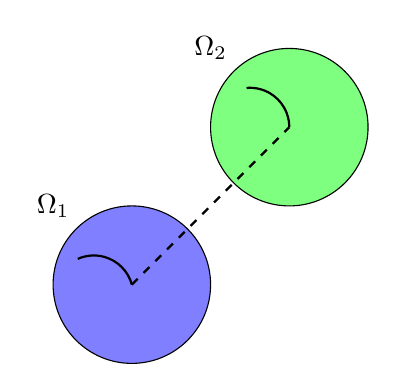
\begin{tikzpicture}
\draw[fill=blue, fill opacity=0.5] (-1,-1) circle (1cm);
\draw (-2,0) node {$\Omega_1$};

\draw[thick] (-1,-1) arc (15:114:0.5);

\draw[fill=green, fill opacity=0.5] (1,1) circle (1cm);
\draw (0,2) node {$\Omega_2$};

\draw[thick] (1,1) arc (0:95:0.5);

\draw[thick, dashed] (-1,-1) -- (1,1);
\end{tikzpicture}
}
\caption[Dos espacios arcoconexos, cada uno conteniendo la imagen de un
símplice singular, junto con una línea discontinua que sale de uno de ellos
para entrar en el otro.]{\labfig{FigPentaHexa}Los arcos de circunferencia son
$1$-símplices singulares de $\Omega$, pero la línea discontinua uniéndolos no
lo es, ya que se sale del espacio.}
\end{marginfigure}

\begin{proposition}
\labprop{SumaDirArco} Sea $X$ un espacio topológico y $\{X_\alpha\colon \alpha
\in A\}$ la familia de arcocomponentes de $X$.
\[H_*(X) \cong \sum_{\alpha \in A} H_*(X_\alpha)\]
\end{proposition}

\begin{proof}
Considérese la aplicación
\begin{diag}
\Psi_k\colon\sum_\alpha S_k(X_\alpha) \arrow[r] & S_k(X)          \\[-0.8cm]
(g_\alpha)_\alpha \arrow[r, maps to]            & \sum_\alpha g_\alpha
\end{diag}

Toda cadena singular $g \in S_k(X)$ admite una descomposición única como
combinación lineal de $k$-símplices singulares. Dado que cada símplice va a parar
a una única componente conexa de $X$, se sigue que
\[\Psi_k(g)=\Psi_k(h) \implies g=h\]
por lo que $\Psi_k$ es inyectiva.

Sea $\phi\colon \sigma_k \to X$ un $k$-símplice singular. Las aplicaciones
continuas preservan la arcoconexión, por lo que $\phi(\sigma_k)$ está en alguna
componente arcoconexa $X_\alpha \subseteq X$. Por tanto, podemos hallar un
$\phi_\alpha \in S_k(X_\alpha)$ tal que
\[\Psi_k(\phi_\alpha)=\phi\]
por lo que $\Psi_k$ es sobreyectiva.

Dado $g=(g_\alpha)_\alpha$,
\[\Psi_k(\p g)=
\Psi_k({\p^\alpha g_\alpha})=
\sum_{\alpha \in A}\p^\alpha g_\alpha=
\p \sum_{\alpha \in A}g_\alpha=\p \Psi_k(g)\]
Se sigue que $\Psi$ es aplicación de cadenas y
\[H_*(X)=H_*[S_*(X)]\cong H_*\left[\sum_{\alpha \in A}S_*(X_\alpha)\right]\]

Finalmente, aplicando \reflemma{HomoSumaDir},
\[H_*\left[\sum_{\alpha \in A}S_*(X_\alpha)\right]\cong
\sum_{\alpha \in A}H_*[S_*(X_\alpha)]=
\sum_{\alpha \in A}H_*\left(X_\alpha\right)\]
\end{proof}
Como consecuencia de este resultado, podemos asumir que todo espacio topológico es
arcoconexo.

Sea $X_\alpha$ una arcocomponente de $X$ y $x,y \in Z_0(X_\alpha)$. Si $a,b \in
\mb{Z}$, $ax+by \in Z_0(X_\alpha)$. Teniendo en cuenta que
\[ax+by=ax+ay-ay+by=a(x-y)+y(a+b)\]
siendo $x-y$ el borde de un 1-símplice y $a+b$ un entero, se tiene que
\[[ax+by]=[a(x-y)+y(a+b)]=a[x-y]+(a+b)[y]=(a+b)[y]\]
Es decir,
\[H_0(X_\alpha)=\la [y]\ra \cong \mb{Z}\]
Si $X$ tiene $n$ arcocomponentes, existirán $y_i \in H_0(X_i)$ ($1 \leq i \leq n$) tales que
\[H_0(X)=\sum^n_{\alpha=1}\la [y_\alpha]\ra\cong
\sum^n_{i=1}\mb{Z} \cong \mb{Z}^n\]

\begin{corollary}
Si $X$ tiene $n$ arcocomponentes,
\[H_0(X)\cong \mb{Z}^n\]
\end{corollary}

\subsection{Homología de un conjunto convexo}
El objetivo de este apartado es probar que todo conjunto convexo tiene el tipo de
homología de un punto. Es decir: si $X$ es un espacio convexo,
\begin{align*}
H_0(X)\cong \mb{Z}; && H_p(X)=0 \quad (p > 0)
\end{align*}
Ya sabemos que $H_0(X)$ tiene un único generador. Por tanto, nos queda probar la
segunda igualdad.

\begin{lemma}\lablemma{ConvexoLema}
Sea $X$ un conjunto convexo. Dado un símplice singular $\phi\colon \sigma_{p} \to
X$, la aplicación $T_p(\phi)\colon \sigma_{p+1} \to X$ dada por
\[(t_0,\dots,t_{p+1})\mapsto
\begin{cases}
\displaystyle(1-t_0)
\phi\left(\frac{t_1}{1-t_0},\dots,\frac{t_{p+1}}{1-t_0}\right)+t_0x
&\mbox{ si }t_0 < 1\\
x & \mbox{ si }t_0=1
\end{cases}\]
es un símplice singular.
\end{lemma}

\begin{proof}
Veamos primero que $T_p(\phi)$ está bien definida: si $t_0 < 1$,
\begin{equation}\label{BienDef}
\sum^{p+1}_{j=0}t_j=
1 \iff \sum^{p+1}_{j=1}t_j=
1-t_0 \iff \sum^{p+1}_{j=1}\frac{t_j}{1-t_0}=1
\end{equation}
por lo que los puntos de la forma $\frac{t_j}{1-t_0}$ están en $\sigma_p$ y
$T_p(\phi)$ está bien definida.

Sea $\tau_j=\frac{t_j}{1-t_0}$. La aplicación $T_p(\phi)$ es claramente continua
en todos los puntos con $t_0 < 1$ por ser composición de funciones continuas.
Pasemos al caso $t_0=1$:
\begin{multline*}
0	\leq \|T_p(\phi)(t_0,\dots,t_{p+1})-x\|=
\|(1-t_0)\phi(\tau_1,\dots,\tau_{p+1})-(1-t_0)x\|\leq\\
	\leq (1-t_0)(\|\phi(\tau_1,\dots,\tau_{p+1})\|+\|x\|)
\end{multline*}

Dado que $\phi$ es continua y $\sigma_p$ es compacto, $\phi(\sigma_p)$ es un
subconjunto compacto de $\mb{R}^n$, por lo que está acotado. Podemos encontrar un
$M > 0$ tal que $\|\phi(\tau_1,\dots,\tau_{p+1})\|$, por lo que
\[0 \leq \|T_p(\phi)(t_0,\dots,t_{p+1})-x\| \leq (1-t_0)(M+\|x\|)\]
De estas desigualdades, concluimos que
\[\lim_{t_0 \to 1}T_p(\phi)(t_0,\dots,t_{p+1})=x\]
y $T_p(\phi)$ es un símplice singular.
\end{proof}

\begin{theorem}\labthm{Convexo}
Sea $X \subset \mb{R}^n$ un conjunto convexo. Dado un $p > 0$,
\[H_p(X)=0\]
\end{theorem}

\begin{proof}
Dado un $p$-símplice singular $\phi$, sea $T_p(\phi)$ el símplice definido en el
lema \reflemma{ConvexoLema}. Queremos ver que
\begin{equation}
\phi=\p T_p(\phi)+T_p(\p \phi) \label{IdTp}
\end{equation}

Por un lado, $\p T_p(\phi)(t_0,\dots,t_p)=\phi(t_0,\dots,t_p)$ por lo que
$\p\circ T_p$ es la identidad. Por otro lado, dado $i=1,\dots,p+1$,
\begin{align*}
T_p(\p_{(i-1)}\phi)(t_0,\dots,t_p)
	&=(1-t_0)(\p_{(i-1)}\phi)(\tau_1,\dots,\tau_p)+t_0x=\\
	&=(1-t_0)\,\phi(\tau_1,\dots,\tau_{i-1},0,\tau_{i-1},\dots,\tau_p)+t_0x=\\
	&=T_p(\phi)(t_0,\dots,t_{i-1},0,t_i,\dots,t_p)=\\
	&=\p_{(i)}T_p(\phi)(t_0,\dots,t_p)
\end{align*}
de forma que $\p_{(i)}(T_p\phi)=T_p(\p_{(i-1)}\phi)$. Combinando ambas
identidades,
\begin{align*}
\p T(\phi)
	&=\p_{(0)}T(\phi)+\sum^{p+1}_{i=1}(-1)^i\partial_{(i)}(T_p\phi)=\\
	&=\phi+\sum^p_{i=0}(-1)^{i+1}T_p(\p_{(i)}\phi)=
	\phi-\sum^p_{i=0}(-1)^iT_p(\p_{(i)}\phi)
\end{align*}
de donde se sigue la identidad deseada.

Sea $z \in Z_p(X)$. Usando \eqref{IdTp}, $z=\p T_p(z)+T_p(\p z)=\p T_p(z)$,
por lo que $z \in B_p(X)$ y
\[H_p(X)=\frac{B_p(X)}{B_p(X)}=0\]
\end{proof}

\section{Homotopías en el grupo de homología}\labsec{HomoHomo}
\begin{definition}
Sea $X$ un espacio topológico. Decimos que $X$ es \textbf{contráctil} si existe
un punto $p \in X$ y una homotopía $F_p$ tal que
\[F_p\colon \id_X \simeq \cte_p\]
\end{definition}

Sea $X$ un espacio contráctil. Por definición, existe un punto $p \in X$ y una
homotopía $F\colon X \times [0,1] \to X$ tales que $F\colon \id_X \simeq
\cte_p$. Si ahora consideramos dos puntos $x,y \in X$, podemos construir el
camino $\alpha\colon [0,1] \to X$ dado por
\[\alpha(t)=
\begin{cases}
F(x,2t) & \text{ si $t < 1/2$}\\
F(y,1-2t) & \text{ si $t \geq 1/2$}
\end{cases}\]

Observamos que $F(x,1)=p=F(y,1)$, de forma que $\alpha$ es continua en
$t=1/2$. Por tanto, podemos hallar un camino que conecta todo par de puntos en
$X$, de forma que $X$ es arcoconexo.

\begin{example}
Sea $A \subseteq \mb{R}^n$ un conjunto convexo. Por ser convexo, dado un $a \in
A$, el segmento $[0,a]$ está contenido en $A$. Eso nos permite definir la
aplicación continua
\begin{diag}
F\colon A\times I \arrow[r] & A                      \\[-0.8cm]
(a,t) \arrow[r, maps to]      & (1-t)a
\end{diag}
por lo que $F\colon \id_A \simeq \cte_0$
\end{example}

\begin{marginfigure}
\resizebox{\textwidth}{!}{
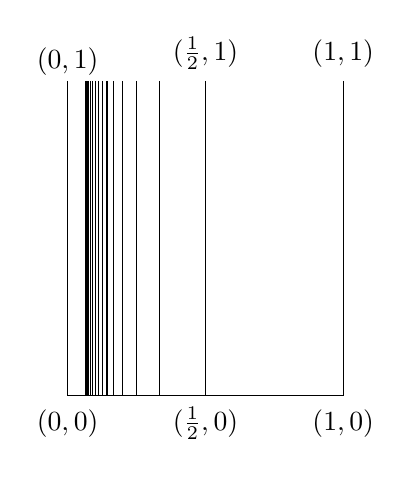
\begin{tikzpicture}
\draw (0,4) -- (0,0) -- (3.5,0);

\foreach \x in {1,...,15}
{
\draw (3.5/\x,4) -- (3.5/\x,0);
}

\draw (3.5,-.35) node {$(1,0)$};
\draw (3.5/2,-.35) node {$(\frac{1}{2},0)$};
\draw (3.5/4,-.35) node {$\hdots$};
\draw (0,-.35) node {$(0,0)$};

\draw (3.5,4.35) node {$(1,1)$};
\draw (3.5/2,4.35) node {$(\frac{1}{2},1)$};
\draw (3.5/4,4.35) node {$\hdots$};
\draw (0,4.25) node {$(0,1)$};
\end{tikzpicture}
}
\caption[Peine del topólogo.]{\labfig{Peine} Primeras $15$ iteraciones del
peine del topólogo. La iteración $w$ añade el segmento correspondiente a
$x=1/w$.}
\end{marginfigure}

\begin{example}
Sea $\Sh$ (pronunciado \emph{sh}) el peine del topólogo. Consideremos la
aplicación continua
\begin{diag}
F\colon \Sh\times I \arrow[r]             & \Sh                   \\[-8mm]
(x,y,t) \arrow[r, maps to] & (x,(1-t)y)
\end{diag}
y la proyección sobre el eje de abscisas, $\pi\colon \mb{R}^2 \to \mb{R}$. La
aplicación $F$ es una homotopía que baja las púas de $\Sh$:
\[F: \id_\Sh \simeq (\pi\times \cte_0)\]
Dado que $\pi \simeq \cte_{(1,0)}$, $\Sh$ es un espacio contráctil.
\end{example}

\begin{definition}
Un subespacio $A$ de $X$ es un \textbf{retracto débil} si podemos hallar una
aplicación continua $r\colon X \to A$ tal que $r|_A\simeq \id_A$. Si podemos
construir $r$ de forma que $r|_A=\id_A$, decimos que $A$ es un \textbf{retracto
fuerte} (o simplemente \textbf{retracto}) y $r$ es una \textbf{retracción}.
\end{definition}

Sea $A$ un retracto de $X$ y $r\colon X \to A$ una retracción. Por definición de
retracto, si $i\colon A \hookrightarrow X$ es la inclusión,
\[r\circ i=\id_A \implies \id_{H_n(A)}=(1_A)_*=(r\circ i)_*=r_*\circ i_*\]
por lo que $r_*$ es sobreyectiva e $i_*$ es inyectiva.

\begin{example}
Sea $D^2$ la bola de centro $p=(0,0)$ y radio 1 de $\mb{R}^2$. Se considera la
aplicación
\begin{diag}
r\colon D^2-\{p\} \arrow[r]             & S^1                   \\[-8mm]
x \arrow[r, maps to] & \frac{x}{\|x\|}
\end{diag}
La aplicación $r$ es continua por ser cociente de funciones continuas. Además,
$r|_{S^1}=\id_{S^1}$. Se sigue que $S^1$ es un retracto de $D^2-\{p\}$.
\end{example}

\begin{example}[\cite{Spanier66}, p. 28]
Sea $X=[0,1]\times[0,1]$ el cuadrado unidad en $\mb{R}^2$. La inclusión $i\colon
\Sh \hookrightarrow X$ define un retracto débil. Sin embargo, se puede probar que
$\Sh$ no es un retracto fuerte de $X$.
\end{example}

\begin{definition}
Sea $A$ un subespacio de $X$. Decimos que $X$ es \textbf{deformable} en $A$ si
existe una aplicación continua $r\colon X \to A$ llamada \textbf{deformación} tal
que $i\circ r \simeq \id_X$, siendo $i\colon A \hookrightarrow X$ la inclusión.
\end{definition}

Dado que $i\circ r\simeq \id_X$, $i_*$ es sobreyectiva y $r_*$ es inyectiva.

\begin{example}\labexample{Deformacion}
\begin{enumerate}
\item Sea $\pi\colon \mb{R}^2 \to \mb{R}$ la proyección sobre el eje de abscisas.
Tomando la aplicación $r(t)=(\cos(2\pi t),\sin(2\pi t))$, se tiene que $r\circ
\pi\colon D^2 \to S^1$ es una deformación. No obstante, si tomamos el punto
$(0,1) \in S^1$,
\[(r\circ \pi)(0,1)=r(0)=(\cos 0,\sin 0)=(1,0)\neq (0,1)\]
por lo que $r\circ \pi$ no es una retracción.
\item Sea $X$ un espacio contráctil a un cierto punto $q$. Si $A$ es un
subespacio de $X$ que contiene a $q$, se tiene que $\cte_q\colon X \to A$ es
una deformación de $X$ en $A$ por definición de espacio contráctil. Por tanto,
$X$ es deformable en cualquier subespacio que contenga a $q$.
\end{enumerate}
\end{example}

\begin{definition}
Decimos que un subespacio $A$ es un \textbf{retracto por deformación fuerte} de
$X$ si podemos hallar una homotopía $F\colon X\times I \to X$ tal que 
\begin{enumerate}
\item dado un $x \in X$, $F(x,0)=x$;
\item $F(X,1) \subseteq A$;
\item dado un $a \in A$ y un $t \in I$, $F(a,t)=a$.
\end{enumerate}
\end{definition}

En particular, observamos que un retracto por deformación fuerte describe
tanto una deformación (ítem 2) como una retracción (ítem 3).

\begin{example}
El peine del topólogo no es un retracto por deformación fuerte del cuadrado
unidad, ya que no es un retracto fuerte.
\end{example}

Sea $i\colon A \hookrightarrow X$ la inclusión. Si $A$ es un retracto por
deformación de $X$, $X$ es deformable en $A$ ($i_*$ es un epimorfismo), pero
$A$ es un retracto de $X$ ($i_*$ es un monomorfismo). Por tanto, se tiene el
siguiente corolario:

\begin{corollary}\label{RDFHomo}
Los retractos por deformación fuerte no alteran el tipo de homología de un
espacio topológico.
\end{corollary}

\subsection{Homotopías de cadenas}
Sean $C$ y $D$ complejos de cadenas, con $f,g\colon C \to D$ aplicaciones de
cadenas. Queremos hallar una condición suficiente para poder afirmar que $f$ y $g$
inducen el mismo homomorfismo entre $H_p(C)$ y $H_p(D)$. Una forma de comprobar
esto es verificar que la aplicación de cadenas $\alpha=f-g\colon C \to D$ induce
el homomorfismo nulo en homologías:
\[f_*=g_* \iff \alpha_*=f_*-g_*=0\]

Sea $c \in Z_p(C) \leq C_p$. Supongamos que existe un $b \in D_{p+1}$ tal que
$\alpha(c)=\p b$. Por cómo se define $B_p(D)$, es inmediato que
\[\alpha_*([c])=[\p b]=0+B_p(D)\]
Existirá una homomorfismo $S\colon C_p \to D_{p+1}$ tal que $\alpha=\p \circ S$.
Pero esta no es una aplicación de cadenas, por lo que no sabemos si va a inducir
un homomorfismo entre los grupos de homología.

Como $S$ es un homomorfismo, $S(0)=0$; así, si tomamos $T=S|_{Z_p(C)}$, se
verifica que $\alpha=\p \circ T + T \circ \p$. Veamos que esta nueva definición
de $\alpha$ conmuta con el operador borde:
\begin{align*}
\p \circ \alpha &=
\p^2 \circ T+\p \circ T \circ \p =
\p \circ T \circ \p=\\
&=\p \circ T \circ \p + T \circ \p^2 =
\alpha \circ \p
\end{align*}

Por construcción, $\alpha_*$ es el homomorfismo nulo. Pero $\alpha=f-g$, por lo
que hemos encontrado una condición suficiente para que $f$ y $g$ induzcan el
mismo homomorfismo entre grupos de homología.

\begin{definition}
Sean $C$ y $D$ complejos de cadenas. Dos aplicaciones de cadenas
$f,g\colon C \to D$ son \textbf{homotópicas} si existe un homomorfismo $T\colon
C \to D$ de grado 1 tal que
\[f-g=\p \circ T+T\circ \p\]
La aplicación $T$ recibe el nombre de \textbf{homotopía de cadenas} entre $f$ y
$g$.
\end{definition}

\subsection{Aplicaciones homotópicas}
\begin{theorem}[Teorema de invarianza homotópica de la homología]
Dadas dos aplicaciones continuas $f,g\colon X \to Y$ homotópicas, $f_*=g_*$.
\end{theorem}

\begin{proof}
Sea $F\colon X \times I \to Y$ una homotopía entre $f$ y $g$. Se definen las
aplicaciones $\alpha,\beta\colon X \to X\times I$ dadas por las expresiones
\begin{align*}
\alpha(x)=(x,0); && \beta(x)=(x,1)
\end{align*}
de forma que $f=F\circ \alpha$ y $g=F\circ \beta$.

Supongamos que existe una homotopía de cadenas $T\colon S_*(X) \to
S_*(X\times I)$ entre $\alpha$ y $\beta$. $T$ induce una homotopía de cadenas
entre $f_\#$ y $g_\#$ de la siguiente forma:
\begin{align*}
f_\#-g_\#&=F_\#\circ\alpha_\#-F_\#\circ\beta_\#=
	F_\#\circ(\alpha_\#-\beta_\#)=\\
	&=F_\#\circ(\p \circ T+T\circ\p)=
	(F_\#\circ\p)\circ T+(F_\#\circ T)\circ\p
\end{align*}
Como $F_\#$ es una aplicación de cadenas,
\begin{align*}
(F_\#\circ\p)\circ T+(F_\#\circ T)\circ\p&=
(\p\circ F_\#)\circ T+(F_\#\circ T)\circ\p=\\
&=\p\circ (F_\#\circ T)+(F_\#\circ T)\circ\p
\end{align*}
por lo que $f_*=g_*$, que es lo que queríamos probar. Por tanto, bastará con
probar que $T$ existe.

Sea $\tau_n\colon \sigma_n \to\sigma_n$ la aplicación identidad. Procedemos a
construir $T$ de forma inductiva: supongamos que $X=\sigma_0$. El símplice
$\sigma_0$ es el espacio puntual formado por el punto 1, de forma que definimos
la 0-cadena
\[c=\alpha_\#(\tau_0)-\beta_\#(\tau_0)=\alpha-\beta \in S_0(\sigma_0\times I)\]
Como $S_0(\sigma_0\times I)=Z_0(\sigma_0\times I)$, $c$ es un 0-ciclo.

Dado que $\sigma_0$ es un espacio puntual, podemos identificar $\alpha$ con
$\alpha(1)=(1,0)$ y $\beta$ con $\beta(1)=(1,1)$. Como $\sigma_0\times I$ es
arcoconexo, existe un camino
\[b\colon I \to \sigma_0\times I\]
tal que $b(0)=(1,0)\equiv \alpha$ y $b(1)=(1,1)\equiv\beta$. Se sigue que $c=
\p b$. Definimos entonces $T_{\sigma_0}(\tau_0):=b$.

Si $X$ es un espacio topológico arbitrario y $\phi\colon \sigma_0 \to X$ un
0-símplice singular, definimos
\[T_X(\phi):=(\phi \times \id_I)_\#(T_{\sigma_0}(\tau_0))\]
La aplicación $T_X$ induce un homomorfismo de $S_0(X)$ en $S_1(X\times I)$ de
forma única.

Sea $X$ un espacio topológico arbitrario y $n > 0$. Supongamos construida para
todo $i < n$ una aplicación $T_X: S_i(X) \to S_{i+1}(X\times I)$ que verifique las
siguientes condiciones:
\begin{enumerate}
\item $\p\circ T_X+T_X\circ\p=\alpha_\#-\beta_\#$ ($\star$) \label{AlfaBetaHomo},
\item $T_X\circ h_\#=(h_\#\times 1_I)\circ T_X$ para toda aplicación continua
$h\colon X \to Y$.
\end{enumerate}

Dado un $d \in S_n(\sigma_n)$, $\p d \in S_{n-1}(\sigma_n)$, por lo que la cadena
singular
\begin{equation}
c=\alpha_\#(d)-\beta_\#(d)-T_{\sigma_n}(\p d)\label{PasoInductivo}
\end{equation}
está bien definida por hipótesis de inducción. Si calculamos $\p c$,
\begin{align*}
\p c&=\p\alpha_\#(d)-\p\beta_\#(d)-\p T_{\sigma_n}(\p d)
\stackrel{\hyperref[AlfaBetaHomo]{(\star)}}{=}\\
	&=\p\alpha_\#(d)-\p\beta_\#(d)-\p\alpha_\#(d)+\p\beta_\#(d)+
	T_{\sigma_n}(\p^2 d)=0
\end{align*}
por lo que $c \in Z_n(\sigma_n\times I)$. Dado que $\sigma_n\times I$ es convexo,
\[H_n(\sigma_n\times I)=
	0 \iff Z_n(\sigma_n\times I)=
	B_n(\sigma_n\times I)\]
por lo que $c \in B_n(\sigma_n\times I)$ Existirá entonces un $b \in
S_{n+1}(\sigma_n\times I)$ tal que $\p b=c$. Se define $T_{\sigma_n}(d)=b$.

Al igual que hicimos en el caso $n=0$, definimos
\[T_X(\phi)=(\phi\times \id_I)_\#(T_{\sigma_n}(\tau_n))\]
Nos queda ver que $T_X$ verifica las dos condiciones descritas en la hipótesis de
inducción.

Veamos que $T_{\sigma_n}$ verifica la condición
$\hyperref[AlfaBetaHomo]{(\star)}$:
\begin{align*}
\p T_{\sigma_n}(d)+T_{\sigma_n}(\p d)&=
\p b+T_{\sigma_n}(\p d)=
c+T_{\sigma_n}(\p d)
\stackrel{\eqref{PasoInductivo}}{=}\\
&=\alpha_\#(d)-\beta_\#(d)-
T_{\sigma_n}(\p d)+T_{\sigma_n}(\p d)=\\
&=\alpha_\#(d)-\beta_\#(d)
\end{align*}
Como la elección de $d$ es arbitraria, se deduce que
$\p\circ T_{\sigma_n}+T_{\sigma_n}\circ\p=\alpha_\#-\beta_\#$.

Sea $\phi\colon \sigma_p \to X$ un $p$-símplice singular. Antes de probar la
primera condición, notar que $\phi_\#(\tau_n)=\phi\circ\tau_n=\phi$, por lo que
\begin{equation}
(T_X\circ\phi_\#)(\tau_n)=T_X(\phi)=(\phi\times 1_I)_\#T_{\sigma_n}(\tau_n)
\label{TConmutaTau}
\end{equation}
De esta forma,
\begin{align*}
\p T_X(\phi)+T_X(\p \phi)
	&=[\p\circ (\phi\times \id_I)_\#\circ T_{\sigma_n}](\tau_n)+
	(T_X\circ\p\circ\phi_\#)(\tau_n)=\\
	&=[\p\circ(\phi\times \id_I)_\#\circ T_{\sigma_n}](\tau_n)+
	(T_X\circ \phi_\#)(\p\tau_n)\stackrel{\eqref{TConmutaTau}}{=}\\[8pt]
	&=[\p\circ(\phi\times \id_I)_\#\circ T_{\sigma_n}](\tau_n)+
	[(\phi\times 1_I)_\#\circ T_{\sigma_n}](\p\tau_n)=\\[8pt]
	&=[(\phi\times \id_I)_\#\circ\p\circ T_{\sigma_n}](\tau_n)+
	[(\phi\times 1_I)_\#\circ T_{\sigma_n}](\p\tau_n)=\\
	&=[(\phi\times \id_I)_\#\circ(\p\circ T_{\sigma_n}+
	T_{\sigma_n}\circ\p)](\tau_n)
	\stackrel{\hyperref[AlfaBetaHomo]{(\star)}}{=}\\[8pt]
	&=(\phi\times \id_I)_\#(\alpha_\#-\beta_\#)(\tau_n)
\end{align*}
Observamos que los diagramas
\begin{center}
\begin{minipage}{0.4\textwidth}
\begin{diag}
\sigma_n \arrow{d}{\phi} \arrow{r}{\alpha} &
\sigma_n\times I \arrow{d}{\phi\times \id_I}\\
X \arrow{r}{\alpha}& X\times I&
\end{diag}
\end{minipage}
%
\begin{minipage}{0.4\textwidth}
\begin{diag}
\sigma_n \arrow{d}{\phi} \arrow{r}{\beta} &
\sigma_n\times I \arrow{d}{\phi\times \id_I}\\
X \arrow{r}{\beta}& X\times I&
\end{diag}
\end{minipage}
\end{center}
son conmutativos, por lo que también conmutan cuando los
convertimos en aplicaciones de cadenas. De aquí se sigue que
\[[(\phi\times \id_I)_\#\circ(\alpha_\#-\beta_\#)](\tau_n)=
[(\alpha_\#-\beta_\#)\circ\phi_\#](\tau_n)=(\alpha_\#-\beta_\#)(\phi)\]
por lo que $\p\circ T_X+T_X\circ\p=\alpha_\#-\beta_\#$.

Para la segunda condición, consideramos $h\colon X \to W$ continua y $\phi \in
S_n(X)$:
\begin{align*}
T_W[h_\#(\phi)]&=
	(T_W \circ h_\#\circ \phi_\#) (\tau_n)=
	[T_W\circ(h\circ \phi)_\#](\tau_n)\stackrel{\eqref{TConmutaTau}}{=}\\[8pt]
	&=[(h\circ\phi)\times \id_I]_\#[T_{\sigma_n}(\tau_n)]=\\[8pt]
	&=[(h\times \id_I)\circ(\phi\times \id_I)]_\#[T_{\sigma_n}(\tau_n)]=\\
	&=[(h\times \id_I)_\#\circ(\phi\times \id_I)_\#][T_{\sigma_n}(\tau_n)]
	\stackrel{\eqref{TConmutaTau}}{=}\\[8pt]
	&=(h\times 1_I)[T_X(\phi)]
\end{align*}
por lo que se cumple la segunda condición.

De esta forma, se construye una homotopía de cadenas entre $\alpha$ y $\beta$.
\end{proof}

Sea $f\colon X \to Y$ una aplicación continua. Decimos que $f$ es una
\textbf{equivalencia de homotopía} si existe una aplicación $g\colon Y \to X$,
llamada \textbf{inversa homotópica}, tal que
\begin{align*}
f\circ g \simeq 1_Y; && g \circ f \simeq 1_X
\end{align*}

\begin{corollary}\label{Contractil}
Si $f\colon X \to Y$ es una equivalencia de homotopía,
\[f_*: H_*(X) \to H_*(Y)\]
es un isomorfismo de grado 0. En particular, si $X$ es un espacio contráctil,
\[H_n(X)\cong H_n(\{\star\})\cong
\begin{cases}
\mb{Z} 	& \text{ si $n=0$}\\
0		& \text{ si $n \neq 0$}
\end{cases}\]
\end{corollary}

\section{Sucesiones exactas}
\begin{definition}
Una colección de grupos y homomorfismos
\[G_0 \xrightarrow{ f_1 } G_1 \xrightarrow{ f_2 } G_2 \xrightarrow{ f_3 }
\dots \xrightarrow{ f_n } G_n\]
es una \textbf{sucesión exacta finita} si $\im f_j=\ker f_{j+1}$ para todo $j$.
\end{definition}

Si $n=4$ y $G_0=0=G_4$, se obtiene una sucesión exacta finita de la forma
\[0 \rightarrow G_1 \xrightarrow{ f_2 } G_2
\xrightarrow{ f_3 } G_3 \rightarrow 0\]
En este caso, hablamos de \textbf{sucesión exacta corta}. Notar que, por
definición de sucesión exacta, $f_2$ es un monomorfismo (su núcleo es el grupo 0)
y $f_3$ es un epimorfismo (su imagen es todo $G_3$).

\begin{definition}
Una colección de grupos y homomorfismos
\[G_0 \xrightarrow{ f_1 } G_1 \xrightarrow{ f_2 } G_2
\xrightarrow{ f_3 } \dots \xrightarrow{ f_n } G_n \xrightarrow{f_{n+1}} \dots\]
es una \textbf{sucesión exacta larga} si $\im f_j=\ker f_{j+1}$ para todo $j$.
\end{definition}

Sean $C,D,E$ complejos de cadenas. Considérese la sucesión exacta corta
\begin{equation}
0 \to C \xrightarrow{ f } D \xrightarrow{ g } E \to 0 \label{SecExactafg}
\end{equation}
siendo $f$ y $g$ aplicaciones de cadenas de grado 0. Por ser aplicaciones de
cadenas, dado un $p \geq 0$, podemos construir el diagrama
\[H_p(C) \xrightarrow{ f_* } H_p(D) \xrightarrow{ g_* } H_p(E)\]
Esta secuencia no es extacta, ya que $f_*$ (resp. $g_*$) podría no ser inyectiva
(resp. sobreyectiva). Lo que sí se cumple es que $\im f_*=\ker g_*$.

Para ver esta identidad, sea $c \in Z_p(C)$. Usando que \eqref{SecExactafg} es
una secuencia exacta,
\[(g\circ f)_*([c])=[(g\circ f)(c)]=0\]
por lo que $\im f_* \leq \ker g_*$.

Análogamente, sea $[z] \in \ker g_* \leq H_p(D)$. Sabemos que $[g(z)]=0$, por
lo que $g(z)=\p d$ para algún $d \in D_{p+1}$. Como $g\colon D_{p+1} \to
E_{p+1}$ es sobreyectivo, podemos hallar un $y \in D_{p+1}$ tal que $d=g(y)$.
Dado que $g$ es aplicación de cadenas,
\[g(z)=\p d=\p g(y)=g(\p y) \implies z-\p y \in \ker g\]

Usando $\ker g=\im f$, existirá un $x \in C_p$ tal que $z-\p y=f(x)$. Como
$[z] \in H_p(D)$, $z \in Z_p(D)$, luego
\[f(\p x)=\p f(x)=\p z-\p^2 y=0 \implies \p x \in \ker f\]
Pero $f$ es un monomorfismo, luego $\p x =0$ y $x \in Z_p(C)$. Esto nos permite
tomar clases módulo $B_p(C)$: usando $f(x)=z-\p y$,
\[f_*([x])=[z-\p y]=[z]\]

Por tanto, $[z] \in \im f_*$, luego $\ker g_* \leq \im f_*$.

Para poder generar una sucesión exacta larga, vamos a introducir un homomorfismo
$\Delta\colon H_*(E) \to H_*(C)$ (llamado \textbf{homomorfismo de conexión}) que
nos permita conectar $H_n(D)$ con $H_{n-1}(C)$. El resultado será una secuencia
exacta
\[\dots \xrightarrow{\Delta} H_n(C) \xrightarrow{ f_* } H_n(D) \xrightarrow{ g_* } H_n(E)
\xrightarrow{ \Delta } H_{n-1}(C)\xrightarrow{f_*}\dots\]

Sea $z \in Z_n(E)$. Como $g\colon D \to E$ es un epimorfismo de grado 0, existe
un $d \in D_n$ tal que $z=g(d)$. Como $z\in \ker \p$ y $g$ es aplicación de
cadenas,
\[g(\p d)=0 \implies \p d \in \ker g=\im f\]
A su vez, $f\colon C \to D$ es un homomorfismo de grado 0. Existirá un $c \in
C_{n-1}$ tal que $\p d=f(c)$. Pero $f$ es aplicación de cadenas inyectiva, por
lo que
\[0=\p d=\p f(c)=f(\p c) \implies c \in \ker f=0 \implies c \in Z_{n-1}(C)\]
Esto define una correspondencia $\delta\colon z \mapsto c$ que depende
implícitamente de $d$.

\begin{proposition}
La aplicación $\Delta\colon H_*(Z) \longrightarrow H_*(C)$ dada por
$\Delta([z])=[\delta c]$ está bien definida y es un homomorfismo.
\end{proposition}

\begin{proof}
Sean $z,z' \in Z_n(E)$ con $z-z' \in B_n(E)$. Existe un $e \in E_{n+1}$ tal que
$\p e=z-z'$.

Sean $d,d' \in D_n$ tales que $g(d)=z$ y $g(d')=z'$, y sean $c,c' \in C_n$ tales
que $\p d=f(c)$ y $\p d'=f(c')$. Dado que $g$ es un epimorfismo, existe un
$a \in D_{n+1}$ tal que $g(a)=e$. Como $g$ es aplicación de cadenas,
\[g(\p a)=\p e=z-z'=g(d-d')\]
de donde se sigue que $d-d'-\p a\in \ker g=\im f$. Podemos elegir entonces un
$b \in C_n$ tal que $f(b)=d-d'-\p a$. Usando que $f$ es aplicación de cadenas,
\[f(\p b)=\p(d-d'-\p a)=\p (d- d')=f(c-c')\]
por lo que $\p b-c-c'\in\ker f$.

Usando que $f$ es inyectiva, concluimos que $c-c'=\p b \in B_{n-1}(C)$.
\end{proof}

\begin{theorem}\labthm{SucExacHomo}
Sean $C, D, E$ complejos de cadenas y
\[0 \to C \xrightarrow{ f } D \xrightarrow{ g } E \to 0\]
una sucesión exacta corta. Si $\Delta\colon H_*(E) \to H_*(C)$ es un homomorfismo
de conexión,
\[H_n(C) \xrightarrow{ f_* } H_n(D) \xrightarrow{ g_* } H_n(E)
\xrightarrow{ \Delta } H_{n-1}(C)\] es una sucesión exacta larga.
\end{theorem}

\begin{proof}
La demostración consiste en dos pasos: probar que $\im g_*=\ker \Delta$ y que
$\im \Delta = \ker f_*$. Empecemos por la primera igualdad: dado un $[z] \in \im
g_*$, existe un $d \in Z_n(D)$ tal que $[g(d)]=[z]$. Dado que $g$ es aplicación
de cadenas y $z$ es un $n$-ciclo,
\[0=\p z=g(\p d) \implies \p d \in \ker g_*=\im f_*\]
Existirá un $c \in C_{n-1}$ de forma que $\p d=f(c)$, por lo que $\Delta([z])=
[c]$. Por otro lado,
\[d \in Z_n(D) \implies \p d=0 \implies f(c)=0\]
pero $f$ es un monomorfismo, así que $c=0$. Esto nos lleva a que $z \in
\ker \Delta$.

Sea $[z] \in \ker \Delta$. Existe un $d \in D_n$ de forma que $g(d)=z$ y $f(c)=
\p d$. En particular, podemos tomar $c=0$, ya que la clase de $c$ será la del 0.
Esto implica que
\[\p d=0 \implies d \in Z_n(D) \iff [d] \in H_n(D)\]
De aquí se sigue que $g_*([d])=[g(d)]=[z]$.

Sea $[c] \in \im \Delta$. Existe un $z \in Z_n(E)$ tal que $[c]=\Delta([z])$, luego
existirá un $d \in D_n$ de forma que $f(c)=d$ y $g(d)=z$. Ahora bien,
\[f(c)= \p d \implies f(c) \in B_n(D) \iff [f(c)]=0\]
Pero $[f(c)]=f_*([c])$, luego $[c] \in \ker f_*$.

Sea $[c] \in \ker f_*$. Sabemos que $f(c) \in B_n(D)$, luego existirá un
$d \in D_n$ tal que $f(c)=\p d$. Sea $z=g(d) \in E_n$. Como $\ker g=\im f$,
$\p z=g(\p d)=(g\circ f)(c)=0$. De aquí se tiene que $z \in Z_n(E)$ y que
\[\Delta([z])=[c] \implies [c] \in \im \Delta\]
\end{proof}
